% Created by tikzDevice version 0.12.3.1 on 2021-12-15 14:08:42
% !TEX encoding = UTF-8 Unicode
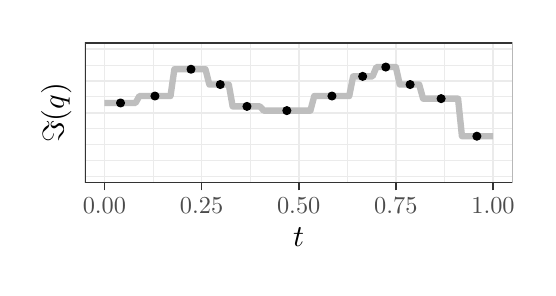
\begin{tikzpicture}[x=1pt,y=1pt]
\definecolor{fillColor}{RGB}{255,255,255}
\path[use as bounding box,fill=fillColor,fill opacity=0.00] (0,0) rectangle (180.67, 86.72);
\begin{scope}
\path[clip] (  0.00,  0.00) rectangle (180.67, 86.72);
\definecolor{drawColor}{RGB}{255,255,255}
\definecolor{fillColor}{RGB}{255,255,255}

\path[draw=drawColor,line width= 0.6pt,line join=round,line cap=round,fill=fillColor] (  0.00,  0.00) rectangle (180.67, 86.72);
\end{scope}
\begin{scope}
\path[clip] ( 20.71, 30.69) rectangle (175.17, 81.22);
\definecolor{fillColor}{RGB}{255,255,255}

\path[fill=fillColor] ( 20.71, 30.69) rectangle (175.17, 81.22);
\definecolor{drawColor}{gray}{0.92}

\path[draw=drawColor,line width= 0.3pt,line join=round] ( 20.71, 38.73) --
	(175.17, 38.73);

\path[draw=drawColor,line width= 0.3pt,line join=round] ( 20.71, 50.21) --
	(175.17, 50.21);

\path[draw=drawColor,line width= 0.3pt,line join=round] ( 20.71, 61.70) --
	(175.17, 61.70);

\path[draw=drawColor,line width= 0.3pt,line join=round] ( 20.71, 73.18) --
	(175.17, 73.18);

\path[draw=drawColor,line width= 0.3pt,line join=round] ( 45.29, 30.69) --
	( 45.29, 81.22);

\path[draw=drawColor,line width= 0.3pt,line join=round] ( 80.39, 30.69) --
	( 80.39, 81.22);

\path[draw=drawColor,line width= 0.3pt,line join=round] (115.50, 30.69) --
	(115.50, 81.22);

\path[draw=drawColor,line width= 0.3pt,line join=round] (150.60, 30.69) --
	(150.60, 81.22);

\path[draw=drawColor,line width= 0.6pt,line join=round] ( 20.71, 32.98) --
	(175.17, 32.98);

\path[draw=drawColor,line width= 0.6pt,line join=round] ( 20.71, 44.47) --
	(175.17, 44.47);

\path[draw=drawColor,line width= 0.6pt,line join=round] ( 20.71, 55.95) --
	(175.17, 55.95);

\path[draw=drawColor,line width= 0.6pt,line join=round] ( 20.71, 67.44) --
	(175.17, 67.44);

\path[draw=drawColor,line width= 0.6pt,line join=round] ( 20.71, 78.93) --
	(175.17, 78.93);

\path[draw=drawColor,line width= 0.6pt,line join=round] ( 27.74, 30.69) --
	( 27.74, 81.22);

\path[draw=drawColor,line width= 0.6pt,line join=round] ( 62.84, 30.69) --
	( 62.84, 81.22);

\path[draw=drawColor,line width= 0.6pt,line join=round] ( 97.94, 30.69) --
	( 97.94, 81.22);

\path[draw=drawColor,line width= 0.6pt,line join=round] (133.05, 30.69) --
	(133.05, 81.22);

\path[draw=drawColor,line width= 0.6pt,line join=round] (168.15, 30.69) --
	(168.15, 81.22);
\definecolor{drawColor}{RGB}{190,190,190}

\path[draw=drawColor,line width= 2.3pt,line join=round] ( 27.74, 59.51) --
	( 29.14, 59.51) --
	( 30.54, 59.51) --
	( 31.95, 59.51) --
	( 33.35, 59.51) --
	( 34.76, 59.51) --
	( 36.16, 59.51) --
	( 37.56, 59.51) --
	( 38.97, 59.51) --
	( 40.37, 62.02) --
	( 41.78, 62.02) --
	( 43.18, 62.02) --
	( 44.59, 62.02) --
	( 45.99, 62.02) --
	( 47.39, 62.02) --
	( 48.80, 62.02) --
	( 50.20, 62.02) --
	( 51.61, 62.02) --
	( 53.01, 71.70) --
	( 54.41, 71.70) --
	( 55.82, 71.70) --
	( 57.22, 71.70) --
	( 58.63, 71.70) --
	( 60.03, 71.70) --
	( 61.44, 71.70) --
	( 62.84, 71.70) --
	( 64.24, 71.70) --
	( 65.65, 66.17) --
	( 67.05, 66.17) --
	( 68.46, 66.17) --
	( 69.86, 66.17) --
	( 71.27, 66.17) --
	( 72.67, 66.17) --
	( 74.07, 58.27) --
	( 75.48, 58.27) --
	( 76.88, 58.27) --
	( 78.29, 58.27) --
	( 79.69, 58.27) --
	( 81.09, 58.27) --
	( 82.50, 58.27) --
	( 83.90, 58.27) --
	( 85.31, 56.75) --
	( 86.71, 56.75) --
	( 88.12, 56.75) --
	( 89.52, 56.75) --
	( 90.92, 56.75) --
	( 92.33, 56.75) --
	( 93.73, 56.75) --
	( 95.14, 56.75) --
	( 96.54, 56.75) --
	( 97.94, 56.75) --
	( 99.35, 56.75) --
	(100.75, 56.75) --
	(102.16, 56.75) --
	(103.56, 62.02) --
	(104.97, 62.02) --
	(106.37, 62.02) --
	(107.77, 62.02) --
	(109.18, 62.02) --
	(110.58, 62.02) --
	(111.99, 62.02) --
	(113.39, 62.02) --
	(114.79, 62.02) --
	(116.20, 62.02) --
	(117.60, 69.12) --
	(119.01, 69.12) --
	(120.41, 69.12) --
	(121.82, 69.12) --
	(123.22, 69.12) --
	(124.62, 69.12) --
	(126.03, 72.49) --
	(127.43, 72.49) --
	(128.84, 72.49) --
	(130.24, 72.49) --
	(131.65, 72.49) --
	(133.05, 72.49) --
	(134.45, 66.17) --
	(135.86, 66.17) --
	(137.26, 66.17) --
	(138.67, 66.17) --
	(140.07, 66.17) --
	(141.47, 66.17) --
	(142.88, 61.08) --
	(144.28, 61.08) --
	(145.69, 61.08) --
	(147.09, 61.08) --
	(148.50, 61.08) --
	(149.90, 61.08) --
	(151.30, 61.08) --
	(152.71, 61.08) --
	(154.11, 61.08) --
	(155.52, 61.08) --
	(156.92, 47.50) --
	(158.32, 47.50) --
	(159.73, 47.50) --
	(161.13, 47.50) --
	(162.54, 47.50) --
	(163.94, 47.50) --
	(165.35, 47.50) --
	(166.75, 47.50) --
	(168.15, 47.50);
\definecolor{drawColor}{RGB}{0,0,0}
\definecolor{fillColor}{RGB}{0,0,0}

\path[draw=drawColor,line width= 0.4pt,line join=round,line cap=round,fill=fillColor] ( 33.56, 59.51) circle (  1.43);

\path[draw=drawColor,line width= 0.4pt,line join=round,line cap=round,fill=fillColor] ( 45.99, 62.02) circle (  1.43);

\path[draw=drawColor,line width= 0.4pt,line join=round,line cap=round,fill=fillColor] ( 59.02, 71.70) circle (  1.43);

\path[draw=drawColor,line width= 0.4pt,line join=round,line cap=round,fill=fillColor] ( 69.58, 66.17) circle (  1.43);

\path[draw=drawColor,line width= 0.4pt,line join=round,line cap=round,fill=fillColor] ( 79.24, 58.27) circle (  1.43);

\path[draw=drawColor,line width= 0.4pt,line join=round,line cap=round,fill=fillColor] ( 93.65, 56.75) circle (  1.43);

\path[draw=drawColor,line width= 0.4pt,line join=round,line cap=round,fill=fillColor] (109.95, 62.02) circle (  1.43);

\path[draw=drawColor,line width= 0.4pt,line join=round,line cap=round,fill=fillColor] (121.05, 69.12) circle (  1.43);

\path[draw=drawColor,line width= 0.4pt,line join=round,line cap=round,fill=fillColor] (129.40, 72.49) circle (  1.43);

\path[draw=drawColor,line width= 0.4pt,line join=round,line cap=round,fill=fillColor] (138.19, 66.17) circle (  1.43);

\path[draw=drawColor,line width= 0.4pt,line join=round,line cap=round,fill=fillColor] (149.40, 61.08) circle (  1.43);

\path[draw=drawColor,line width= 0.4pt,line join=round,line cap=round,fill=fillColor] (162.32, 47.50) circle (  1.43);
\definecolor{drawColor}{gray}{0.20}

\path[draw=drawColor,line width= 0.6pt,line join=round,line cap=round] ( 20.71, 30.69) rectangle (175.17, 81.22);
\end{scope}
\begin{scope}
\path[clip] (  0.00,  0.00) rectangle (180.67, 86.72);
\definecolor{drawColor}{gray}{0.20}

\path[draw=drawColor,line width= 0.6pt,line join=round] ( 27.74, 27.94) --
	( 27.74, 30.69);

\path[draw=drawColor,line width= 0.6pt,line join=round] ( 62.84, 27.94) --
	( 62.84, 30.69);

\path[draw=drawColor,line width= 0.6pt,line join=round] ( 97.94, 27.94) --
	( 97.94, 30.69);

\path[draw=drawColor,line width= 0.6pt,line join=round] (133.05, 27.94) --
	(133.05, 30.69);

\path[draw=drawColor,line width= 0.6pt,line join=round] (168.15, 27.94) --
	(168.15, 30.69);
\end{scope}
\begin{scope}
\path[clip] (  0.00,  0.00) rectangle (180.67, 86.72);
\definecolor{drawColor}{gray}{0.30}

\node[text=drawColor,anchor=base,inner sep=0pt, outer sep=0pt, scale=  0.88] at ( 27.74, 19.68) {0.00};

\node[text=drawColor,anchor=base,inner sep=0pt, outer sep=0pt, scale=  0.88] at ( 62.84, 19.68) {0.25};

\node[text=drawColor,anchor=base,inner sep=0pt, outer sep=0pt, scale=  0.88] at ( 97.94, 19.68) {0.50};

\node[text=drawColor,anchor=base,inner sep=0pt, outer sep=0pt, scale=  0.88] at (133.05, 19.68) {0.75};

\node[text=drawColor,anchor=base,inner sep=0pt, outer sep=0pt, scale=  0.88] at (168.15, 19.68) {1.00};
\end{scope}
\begin{scope}
\path[clip] (  0.00,  0.00) rectangle (180.67, 86.72);
\definecolor{drawColor}{RGB}{0,0,0}

\node[text=drawColor,anchor=base,inner sep=0pt, outer sep=0pt, scale=  1.10] at ( 97.94,  7.64) {$t$};
\end{scope}
\begin{scope}
\path[clip] (  0.00,  0.00) rectangle (180.67, 86.72);
\definecolor{drawColor}{RGB}{0,0,0}

\node[text=drawColor,rotate= 90.00,anchor=base,inner sep=0pt, outer sep=0pt, scale=  1.10] at ( 13.08, 55.95) {$\Im(q)$};
\end{scope}
\end{tikzpicture}
